\documentclass[12pt]{article}
\usepackage{amsmath}
\usepackage{booktabs}
\usepackage{geometry}
\geometry{a4paper, margin=1in}
\usepackage{ctex} % 支持中文
\setCJKmainfont{SimSun} % 设置中文字体,例如宋体
\usepackage{natbib} % 用于引用

\usepackage{svg}

\title{基于颅内血流动力学的脑灌注模型的生理控制策略}
\author{}
\date{March 2025}

\begin{document}



\begin{abstract}
    自体血脑灌注有望被用于治疗缺血性脑卒中,延长治疗时间窗。
    在本研究中,首先建立了基于颅内血流动力学与血泵的脑灌注耦合模型,然后通过仿真结合不同的生理控制策略讨论了脑灌注评价指标,并提出了一种脉动流血泵控制策略。
    最后仿真结果显示,脉动流生理控制策略在保持最佳灌注压的同时能有效提高血管搏动性。

\end{abstract}

\section{引言}
脑卒中是工业化国家中第二大死亡原因,也是导致致残和功能障碍的首要原因。由于缺血性脑卒中治疗具有时间敏感性,延迟会显著影响预后,因此自体血脑灌注结合机械取栓可用于治疗缺血性脑卒中,延长治疗时间窗,挽救缺血半暗带。
在本研究中,实现自体血脑灌注的方法是将血流从患者右侧大腿股动脉引出,经过氧合、降温等措施后由血泵作为脑辅助灌注装置通过介入导管从患者左侧股动脉将血液输送至颈内动脉。
在此构想下,基于颅内血流动力学原理建立颅内-血泵耦合模型,结合颅内血流动力学参数指标设计了脉动流的血泵控制策略,通过仿真实现了在保持最佳脑灌注的同时提升了血管搏动性,减少并发症。

\section{颅内-血泵耦合模型的建立}
基于Ursino-Lodi的颅内血流动力学简化模型,建立图1所示的颅内血流动力学-血泵耦合模型。图中左侧H圆代表心脏,其上方P圆代表血泵,两个压力源合成为系统动脉压$Pa$,其总和的流量$Q = Q_h + Q_p$通过此电学类比模型可分析调节血泵转速对颅内各种参数的影响。

\begin{figure}[h]
    \centering
    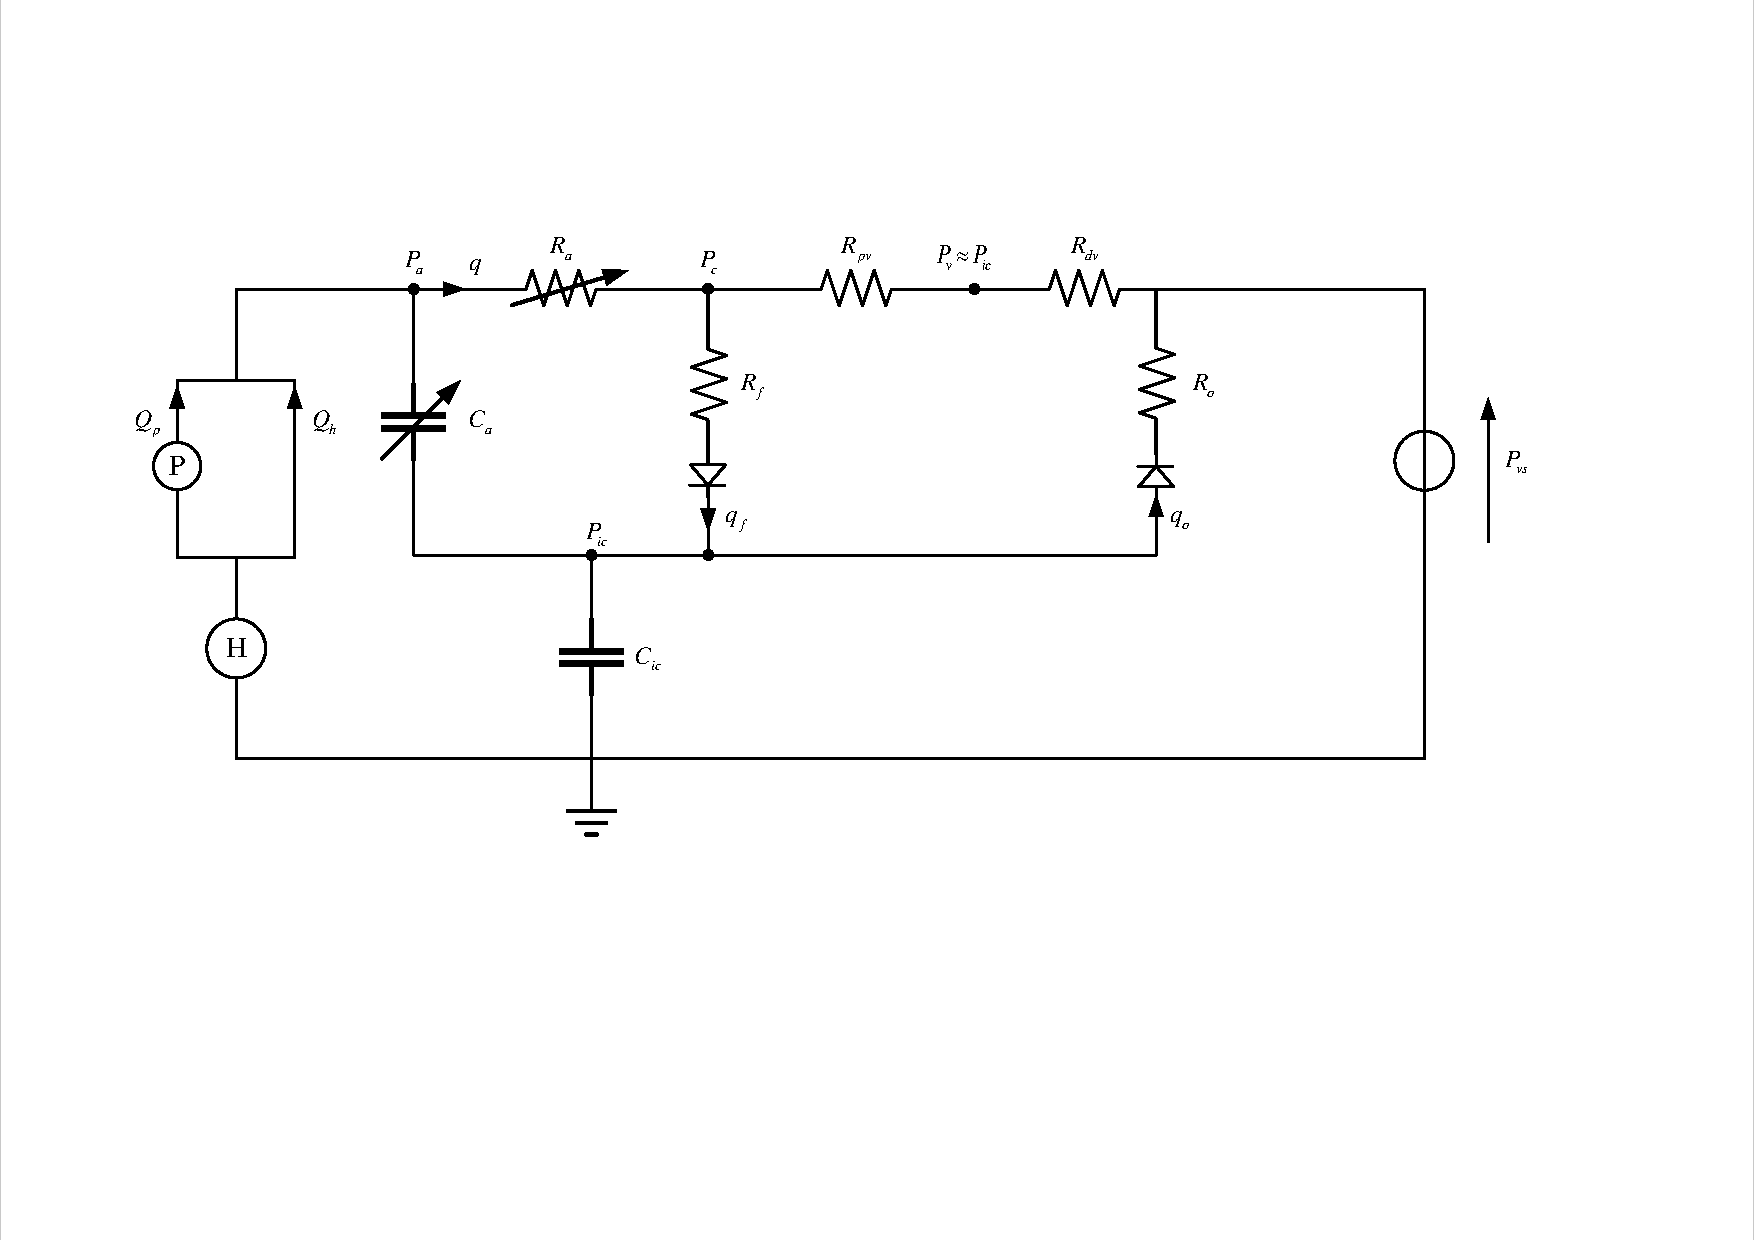
\includegraphics[width=0.8\textwidth]{figures/基于颅内压指标的脑灌注模型.pdf}
    \caption{模型参数包括脑自动调节控制的动脉阻力$R_a$和顺应性$C_a$,静脉侧分别由近端和远端阻力$R_{pv}$和$R_{dv}$以及静脉压力$P_v$建模。脑脊液(CSF)通过$R_f$从大脑脑室中的脉络丛产生,然后通过$R_o$重新被静脉窦吸收。颅内压和颅内顺应性分别表示为$P_{ic}$和$C_{ic}$。}
    \label{fig:brain_perfusion_model}
\end{figure}
\section{颅内-血泵耦合模型仿真验证}


\section{仿真验证}
上述最优解的设计螺旋角进行了重新建模,然后进行了CFD仿真验证,如图4所示。拟合模型的预测值和CFD计算结果如表\ref{tab:comparison}所示。流量差异为1.6\%,溶血率差异为2.6\%。

\begin{table}[h]
    \centering
    \caption{Comparison Between Fitting Model and CFD Calculation}
    \label{tab:comparison}
    \begin{tabular}{lcc}
        \toprule
        Item & Flow rate (ml/min) & Hemolysis rate \\
        \midrule
        Predicted value & 271.0 & $1.19 \times 10^{-4}$ \\
        CFD value & 275.6 & $1.16 \times 10^{-4}$ \\
        Previous value & 215.5 & $5.42 \times 10^{-4}$ \\
        \bottomrule
    \end{tabular}
\end{table}

\section{结论}
仿真结果验证了优化方法的准确性和优势。与原始泵相比,流量增加了27.9\%,溶血率降低了78.6\%。



\end{document}